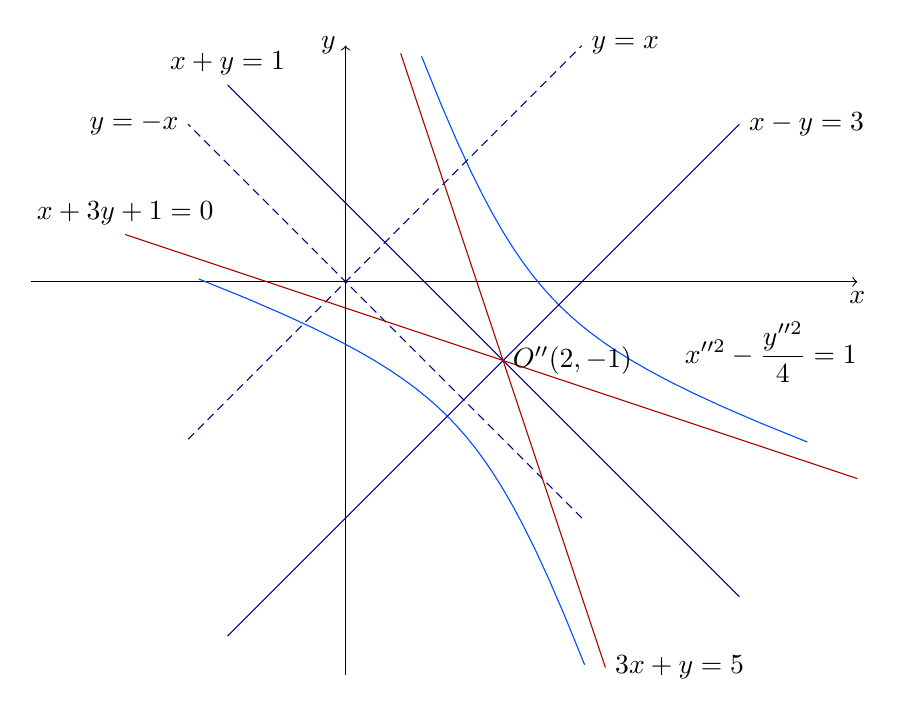
\begin{tikzpicture}[every node/.style={black}]
  \draw [->] (-4,0) -- (6.5,0) node [below] {$x$};
  \draw [->] (0,-5) -- (0,3) node [left] {$y$};
  \begin{scope}[shift = {(2,-1)},blue!70!cyan]
    \draw [rotate = 45,domain=-60:60] plot ({sec(\x)},{2*tan(\x)});
    \draw [rotate = 45,domain=-60:60] plot ({-sec(\x)},{2*tan(\x)});
  \end{scope}
  \draw [blue!50!black] plot[domain=-1.5:5] (\x,\x-3) node[right] {$x-y=3$}
  plot[domain = 5:-1.5] (\x,1-\x)node[above] {$x+y=1$};
  \draw [densely dashed,blue!50!black,domain = -2:3] plot[domain = 3:-2] (\x,-\x)node[left] {$y=-x$} plot(\x,\x) node[right]{$y=x$};
  \draw [red!70!black] plot [domain = -2.5:0.6] (-3*\x-1,\x) node[above] {$x+3y+1=0$}
  plot [domain = 0.7:3.3] (\x,5-3*\x) node [right]{$3x+y=5$};
  \node at (5.4,-0.9) {$\displaystyle x''^2-\frac{y''^2}4=1$};
  \node [right] at (2,-1) {$O''(2,-1)$};
\end{tikzpicture} 